% \documentclass[a4paper,12pt]{article}

% % Paquetes básicos
% \usepackage[utf8]{inputenc}
% \usepackage[T1]{fontenc}
% \usepackage[spanish]{babel}
% \usepackage{graphicx}
% \usepackage{xcolor}
% \usepackage{lipsum}
% \usepackage{geometry}
% \geometry{top=3cm, bottom=3cm, left=2.5cm, right=2.5cm}

% % Paquetes para diseño
% \usepackage{titlesec}
% \usepackage{fancyhdr}
% \usepackage{amsmath}
% \usepackage{amssymb}
% \usepackage{hyperref}

% % Paquetes para el entorno lstlisting
% \usepackage{listings}
% \usepackage{inconsolata}

% % Paquete para fondo
% \usepackage{background}

% % Configuración de lstlisting
% \lstset{
%     language=Python,
%     basicstyle=\ttfamily\small,
%     keywordstyle=\color{blue}\bfseries,
%     stringstyle=\color{teal},
%     commentstyle=\color{gray}\itshape,
%     numbers=left,
%     numberstyle=\tiny\color{gray},
%     backgroundcolor=\color{black!5},
%     frame=single,
%     rulecolor=\color{black!50},
%     breaklines=true,
%     captionpos=b,
%     showstringspaces=false
% }

% % Configuración de título
% \titleformat{\section}{\normalfont\Large\bfseries}{\thesection}{1em}{}
% \usepackage{mathpazo}

% %encabezado y pie de página nivel profesional
% \usepackage{fancyhdr}
% \pagestyle{fancy}
% \fancyhf{}
% \fancyhead[L]{\leftmark}
% \fancyhead[R]{\rightmark}
% \fancyfoot[C]{\thepage}
% \fancyfoot[R]{\textbf{       (UGR)} \today}



% % Información del documento
% \title{
%     \vspace{-2cm}
%     
\includegraphics[width=0.3\textwidth]{images/fccee.jpg} \\ % Cambia el logo si es necesario
%     \LARGE Ingeniería Informática + ADE\\
%     \large Universidad de Granada (UGR)\\[1cm]
% }
% \author{\textbf{Autor:} Ismael Sallami Moreno}
% \date{\textbf{Asignatura:} Resolución de los Ejercicios Propuestos Reueltos Tema 5: Inmovilizaciones materiales}

% % Configuración del fondo
% \backgroundsetup{
%     scale=1,
%     color=black,
%     opacity=0.2,
%     angle=0,
%     position=current page.south,
%     vshift=0pt,
%     hshift=0pt,
%     contents={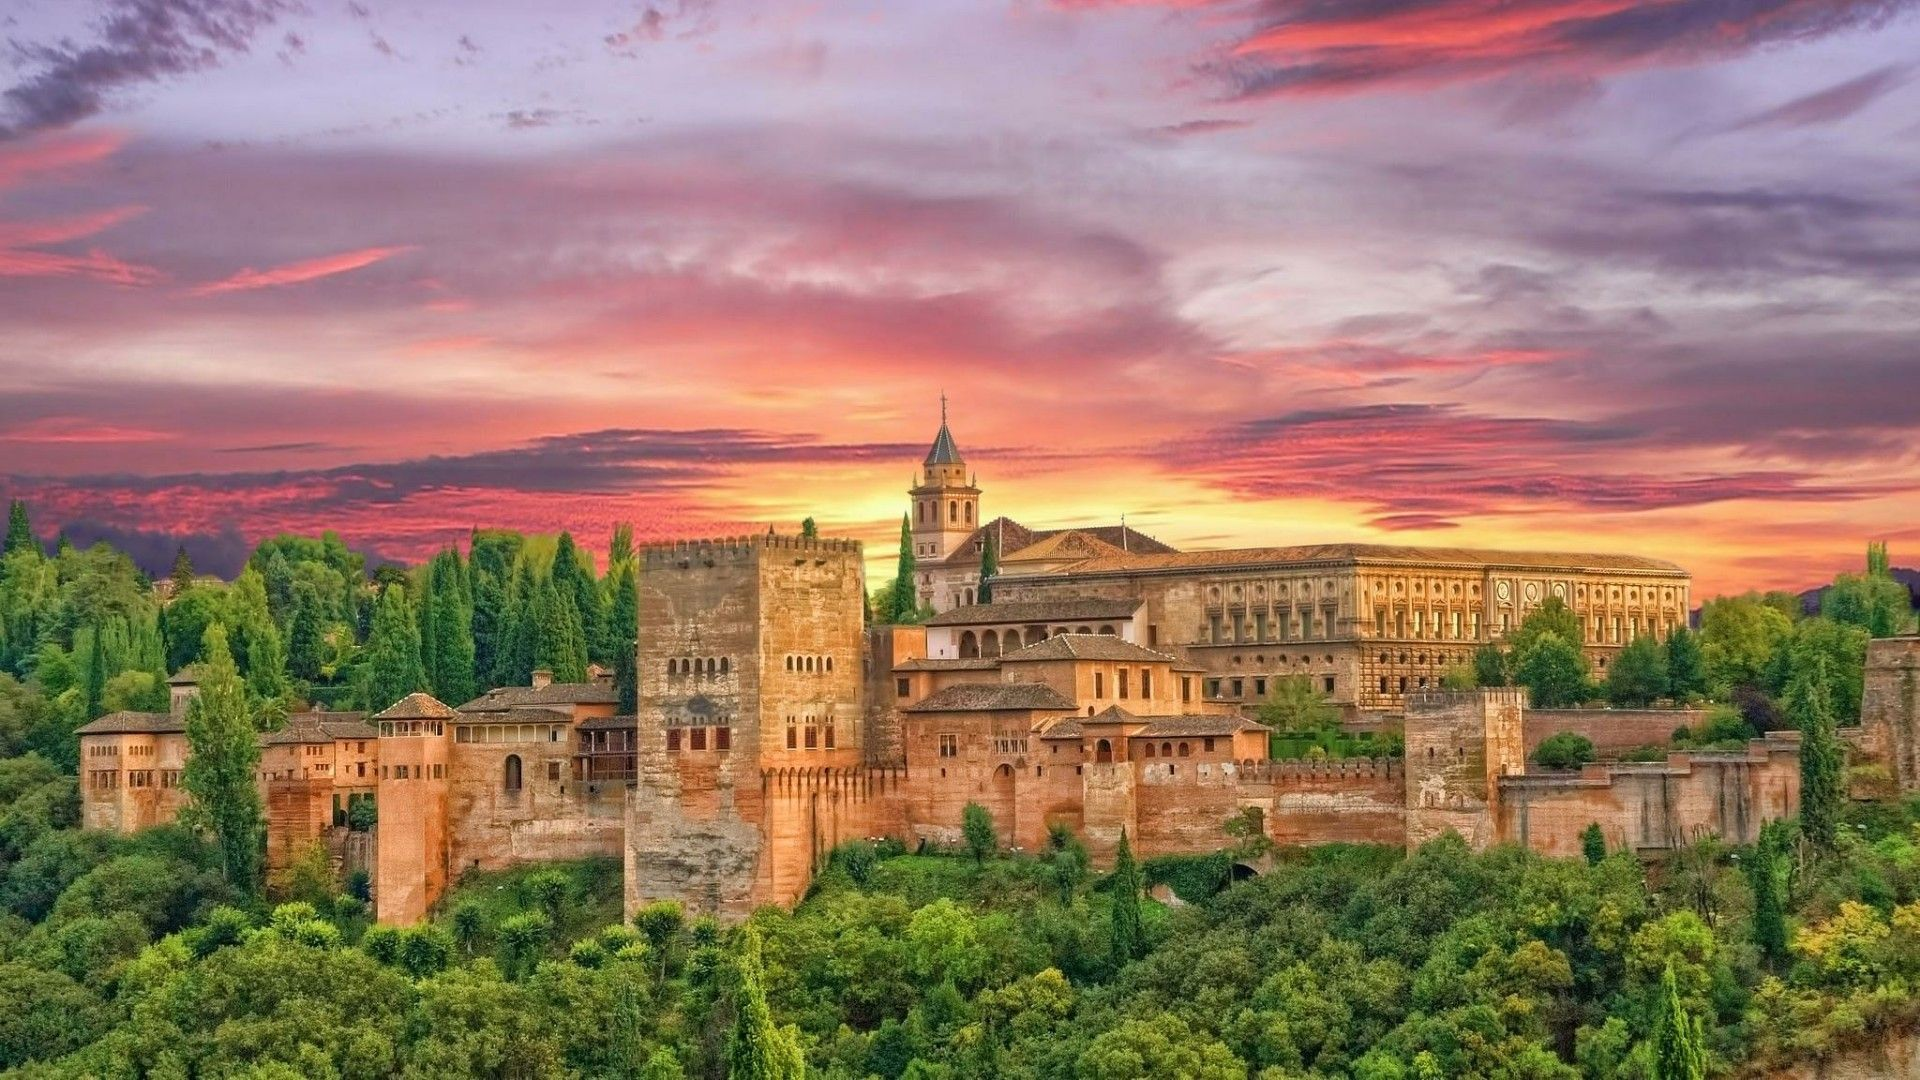
\includegraphics[width=\paperwidth,height=\paperheight,keepaspectratio]{images/granada.jpg}}
% }


\documentclass[a4paper,12pt]{article}

% Paquetes básicos
\usepackage[utf8]{inputenc}
\usepackage[T1]{fontenc}
\usepackage[spanish]{babel}
\usepackage{graphicx}
\usepackage{xcolor}
\usepackage{lipsum}
\usepackage{geometry}
\geometry{top=3cm, bottom=3cm, left=2.5cm, right=2.5cm}

% Paquetes para diseño
\usepackage{titlesec}
\usepackage{fancyhdr}
\usepackage{amsmath}
\usepackage{amssymb}
\usepackage{hyperref}
\usepackage{tcolorbox}
\usepackage{float}

% Paquetes para el entorno lstlisting
\usepackage{listings}
\usepackage{inconsolata}

\usepackage{tocbibind} % Para incluir subsubsubsections en el índice
\usepackage{titlesec}  % Para ajustar la numeración de las secciones
\setcounter{tocdepth}{5} % Ajusta la profundidad del índice
\setcounter{secnumdepth}{5} % Ajusta la profundidad de la numeración

% Configuración de la numeración para \paragraph
\titleformat{\paragraph}
{\normalfont\normalsize\bfseries}{\theparagraph}{1em}{}
\titlespacing*{\paragraph}{0pt}{3.25ex plus 1ex minus .2ex}{1.5ex plus .2ex}

% Paquete para fondo
\usepackage{background}

\newcommand{\fec}{31/12/}
\newcommand{\AIM}{681 Amortización del inmovilizado material }
\newcommand{\AAMAQ}{2813 Amortización acumulada de maquinaria }
\newcommand{\valorrecuperable}{Valor recuperable = max\{valor neto realizable, valor en uso\} =}
\newcommand{\PDI}{691 Pérdidas por deterioro de inmovilizado material}
\newcommand{\DVM}{2913 Deterioro del valor de la maquinaria }
\newcommand{\RDIM}{791 Reversión deterioro inmovilizado material}
\newcommand{\VC}{Valor contable = }
\newcommand{\PPIM}{671 Pérdidas procedentes del inmovilizado material}
\newcommand{\bancos}{572 Bancos cuenta corriente}
\newcommand{\cuotaamort}{Cuota de amortización = }
\newcommand{\enajenacion}{543 Créditos a corto plazo por enajenación del inmovilizado}
\newcommand{\benefIM}{771 Beneficios procedentes del inmovilizado material}
\usepackage{amsmath}
\newcommand{\myequation}[2]{\ensuremath{\frac{#1}{#2}}}
\newcommand{\flechita}{$\rightarrow$}
\newcommand{\deterioropatente}{2903 Deterioro de valor de la propiedad industrial}
\newcommand{\perdidasdelintangible}{690 Pérdidas por inmovilizado intangible}
\newcommand{\amortAcumPatente}{2803 Amortización acumulada de la propiedad industrial}
\newcommand{\trabajosrealizadosII}{730 Trabajos realizados para el inmovilizado intangible}
\newcommand{\cursiva}[1]{\textit{#1}}
\newcommand{\negrita}[1]{\textbf{#1}}
%comandos extra
% \newcommand{\cuenta2800}{2800. Amortización acumulada de investigación}
% \newcommand{\cuenta2801}{2801. Amortización acumulada de desarrollo}
% \newcommand{\cuenta2802}{2802. Amortización acumulada de concesiones administrativas}
% \newcommand{\cuenta2803}{2803. Amortización acumulada de propiedad industrial}
% \newcommand{\cuenta2805}{2805. Amortización acumulada de derechos de traspaso}
% \newcommand{\cuenta2806}{2806. Amortización acumulada de aplicaciones informáticas}
% \newcommand{\cuenta2811}{2811. Amortización acumulada de construcciones}
% \newcommand{\cuenta2812}{2812. Amortización acumulada de instalaciones técnicas}
% \newcommand{\cuenta2813}{2813. Amortización acumulada de maquinaria}
% \newcommand{\cuenta2814}{2814. Amortización acumulada de utillaje}
% \newcommand{\cuenta2815}{2815. Amortización acumulada de otras instalaciones}
% \newcommand{\cuenta2816}{2816. Amortización acumulada de mobiliario}
% \newcommand{\cuenta2817}{2817. Amortización acumulada de equipos para procesos de información}
% \newcommand{\cuenta2818}{2818. Amortización acumulada de elementos de transporte}
% \newcommand{\cuenta2819}{2819. Amortización acumulada de otro inmovilizado material}
% \newcommand{\cuenta282}{282. Amortización acumulada de las inversiones inmobiliarias}


% Configuración de lstlisting
\lstset{
    language=Python,
    basicstyle=\ttfamily\small,
    keywordstyle=\color{blue}\bfseries,
    stringstyle=\color{teal},
    commentstyle=\color{gray}\itshape,
    numbers=left,
    numberstyle=\tiny\color{gray},
    backgroundcolor=\color{black!5},
    frame=single,
    rulecolor=\color{black!50},
    breaklines=true,
    captionpos=b,
    showstringspaces=false
}

% Configuración de título
\titleformat{\section}{\normalfont\Large\bfseries}{\thesection}{1em}{}

% Información del documento
\title{
    \vspace{-2cm}
    
\includegraphics[width=0.3\textwidth]{images/fccee.jpg} \\ % Cambia el logo si es necesario
    \LARGE Ingeniería Informática + ADE\\
    \large Universidad de Granada (UGR)\\[1cm]
}
\author{\textbf{Autor:} Ismael Sallami Moreno}
\date{\textbf{Asignatura:} Resolución de los Ejercicios Propuestos Reueltos Tema 6: Inmovilizado Intangible
}
\usepackage{mathpazo}
\usepackage{fancyhdr}
\pagestyle{fancy}
\fancyhf{}
\fancyhead[L]{\leftmark}
\fancyhead[R]{\rightmark}
\fancyfoot[C]{\thepage}
\fancyfoot[R]{\textbf{       (UGR)} \today}
\usepackage{enumitem}

\usepackage{tcolorbox}

% Configuración del fondo
\backgroundsetup{
    scale=1,
    color=black,
    opacity=0.2,
    angle=0,
    position=current page.south,
    vshift=0pt,
    hshift=0pt,
    contents={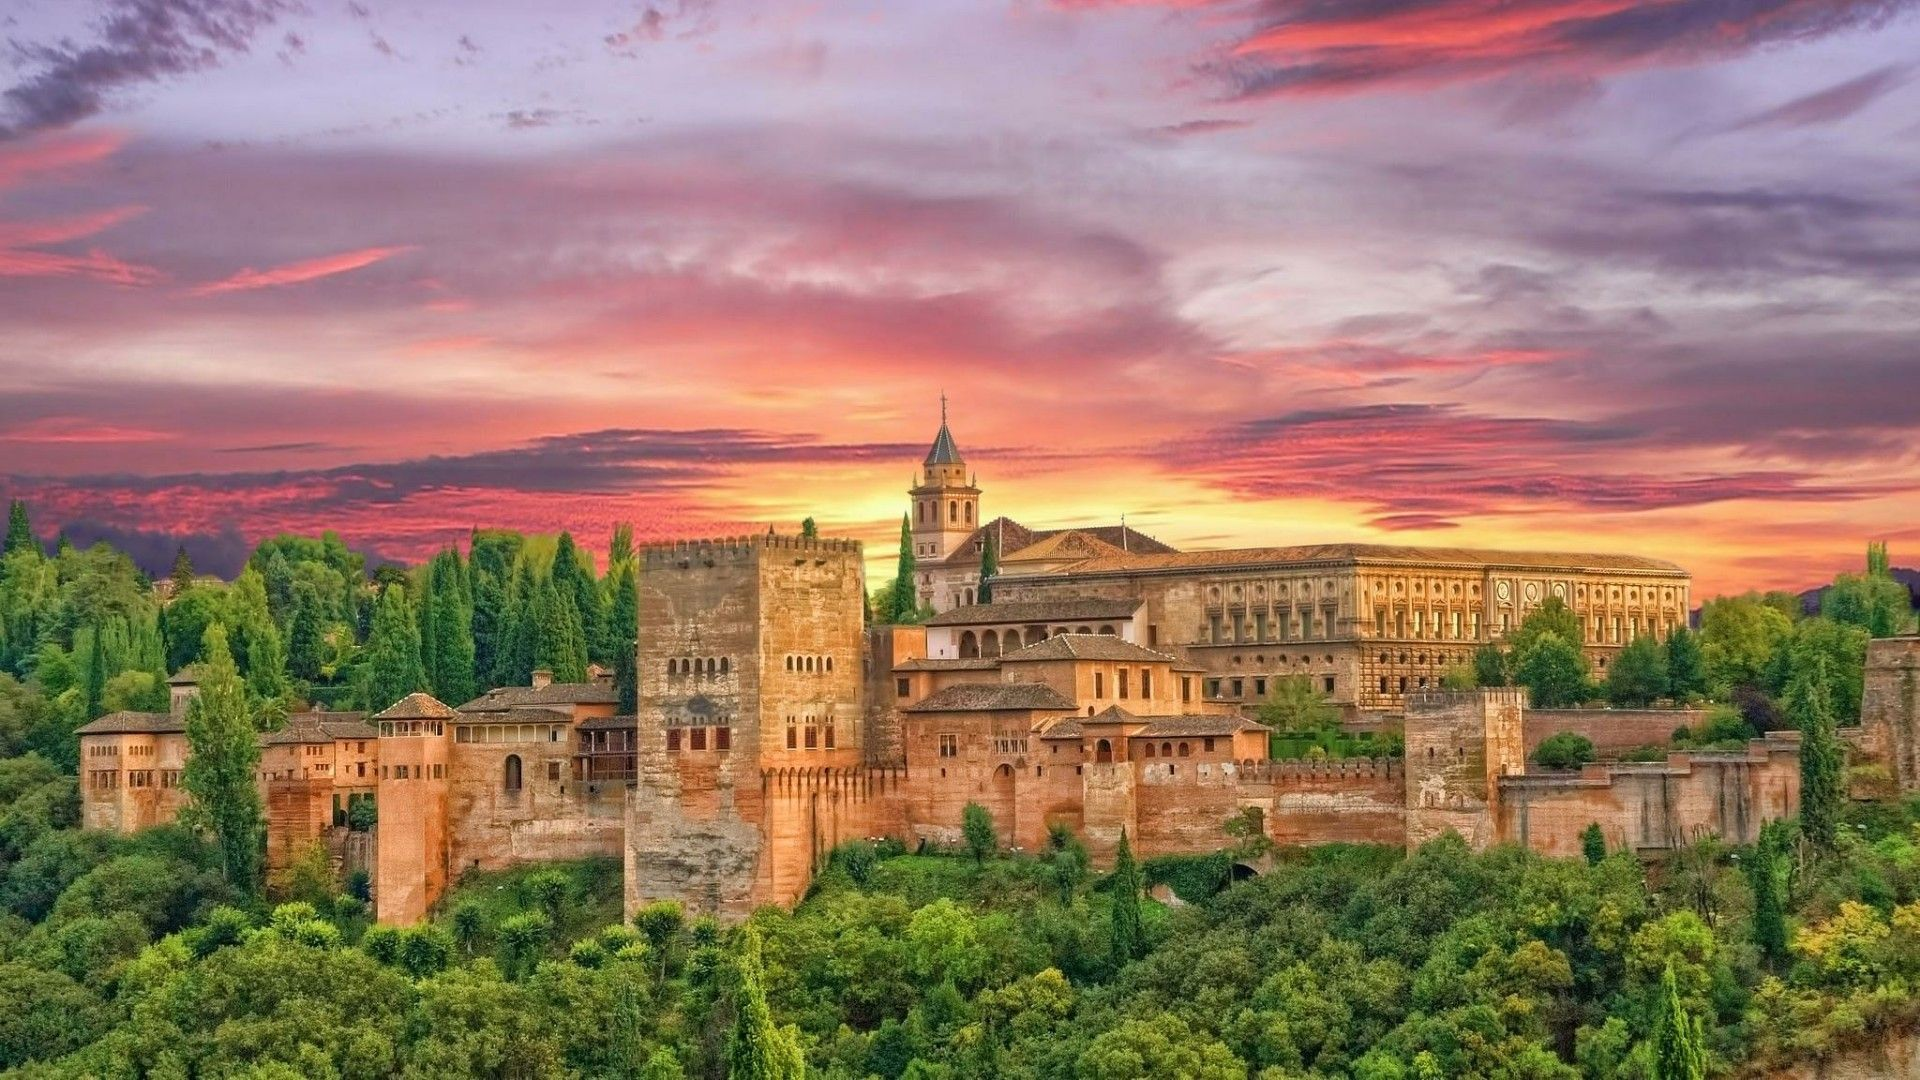
\includegraphics[width=\paperwidth,height=\paperheight,keepaspectratio]{images/granada.jpg}}
}

% Inicio del documento
\begin{document}

% Portada
\maketitle
\thispagestyle{empty}

\begin{center}
    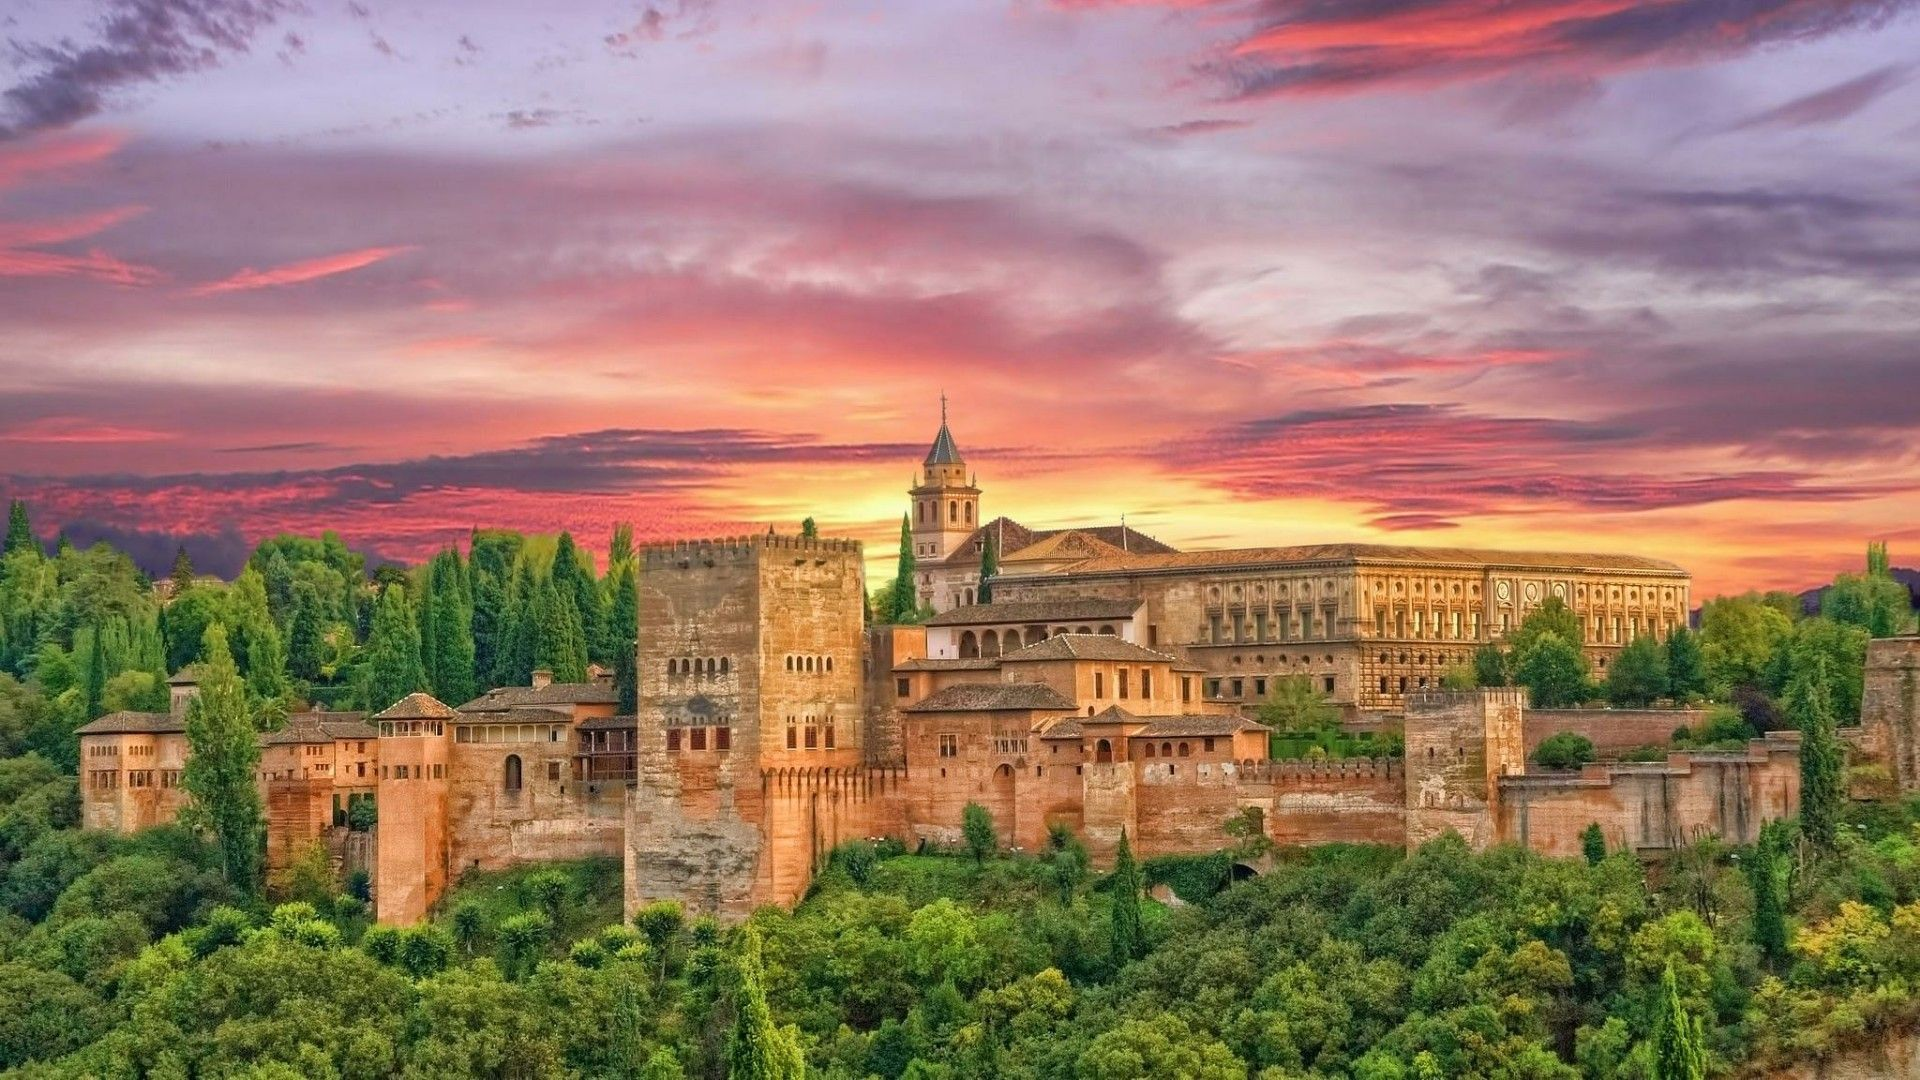
\includegraphics[width=\textwidth,height=0.4\textheight,keepaspectratio]{images/granada.jpg} \\ % Añade tu imagen de fondo
    \vfill
\end{center}

\newpage

% Índice (opcional)
\tableofcontents
\newpage

\section{Ejercicio 1}

\begin{table}[H]
    \centering
    \begin{tabular}{|p{3cm}|p{6cm}|p{3cm}|}
    \hline
    \textbf{DEBE} & \textbf{operaciones de la compra de la patente a 1/10/2017} & \textbf{HABER} \\
    \hline
    175.000 & 203  Propiedad industrial & \\
    \hline
    & \bancos & 175.000\\
    \hline
    \end{tabular}
\end{table}

\begin{itemize}
    \item \valorrecuperable \{114.00, 110.000\} = 114.000
    \item \textbf{La vida útil de la patente se acorta a 3 años a partir de este momento}
    \item \cuotaamort \myequation{200000}{8} = 25.000
    \item \VC 200.000 - 25.000·\myequation{3}{12}(2017) - 25.000 (2018) - 25.000 (2019) - 25.000 (2020) = 118.750
    \item Deterior de la patente = 118.750 - 114.000 = 4.750
\end{itemize}

\begin{table}[H]
    \centering
    \begin{tabular}{|p{3cm}|p{6cm}|p{3cm}|}
    \hline
    \textbf{DEBE} & \textbf{correción valorativa de carácter reversible el 31/12/2020} & \textbf{HABER} \\
    \hline
    4750& 690 Pérdidas por inmovilizado intangible& \\
    \hline
    & 2903 Deterioro de valor de la propiedad industrial&4750 \\
    \hline
    \end{tabular}
\end{table}

\begin{itemize}
    \item Al haber deterioro debemos de recalcular el valor de la amortización.
    \item Los meses que quedan son: 96 (8 años) - los tres años amortizados 3*12 - 3 meses de 2017 = 57 meses 
    % \item \cuotaamort 118.750 - 4750 = \myequation{114000}{57 \text{ meses}} = 2000 cada mes 
    %\item De 2021 han pasado 6 meses, por lo que la amortización de 2021 es 2000·6 = 12.000
    \item \cuotaamort \myequation{114000}{3} = 38.000 cada año
    \item De 2021 han pasado 6 meses, por lo que la amortización de 2021 es 38.000/2 = 19.000
    \item La Amortización total de la patente es = 200.000 - 118.750 = 81.250 + (la de 2021) = 81.250 + 19.000 = 100.250 
\end{itemize}

\begin{table}[H]
    \centering
    \begin{tabular}{|p{3cm}|p{6cm}|p{3cm}|}
    \hline
    \textbf{DEBE} & \textbf{venta de la patente el 1/7/2021} & \textbf{HABER} \\
    \hline
    100.250 & 2803 Amortización acumulada de la propiedad industrial& \\
    \hline
    4.750 & 2903 Deterioro de valor de la propiedad industrial& \\
    \hline
    100.000& \bancos & \\
    \hline
    & 203 Propiedad Industrial& 200.000\\
    \hline
    & \textbf{770 Beneficios procedentes del Inmovilizado Intangible}& 5.000\\
    \hline
    \end{tabular}
\end{table}

\section{Ejercicio 2}

\begin{table}[H]
    \centering
    \begin{tabular}{|p{3cm}|p{6cm}|p{3cm}|}
    \hline
    \textbf{DEBE} & \textbf{a \fec2016 activación de gastos imputables al Proyecto A} & \textbf{HABER} \\
    \hline
    10.000 & 620 gastos de investigación y desarollo del ejercicio& \\
    \hline
    & \bancos & 10.000\\
    \hline
    10.000& 200 Investigación& \\
    \hline
    & 730 Trabajos realizados para el inmovilizado intangible&  10.000\\
    \hline
    \end{tabular}
\end{table}



\begin{table}[H]
    \centering
    \begin{tabular}{|p{3cm}|p{6cm}|p{3cm}|}
    \hline
    \textbf{DEBE} & \textbf{a \fec2017 activación de los gastos imputables al Proyecto B} & \textbf{HABER} \\
    \hline
    2.500 & 620 gastos de investigación y desarollo del ejercicio& \\
    \hline
    & \bancos & 2.500\\
    \hline
    2.500& 200 Investigación& \\
    \hline
    & 730 Trabajos realizados para el inmovilizado intangible&  2.500\\
    \hline
    \end{tabular}
\end{table}

\begin{itemize}
    \item \cuotaamort \myequation{2500}{5 \text{ años}} = 500
\end{itemize}

\begin{table}[H]
    \centering
    \begin{tabular}{|p{3cm}|p{6cm}|p{3cm}|}
    \hline
    \textbf{DEBE} & \textbf{a \fec2019 Amortización EXCLUSIVAMENTE de los gastos del desarollo del Proyecto A} & \textbf{HABER} \\
    \hline
    500 & 680 Amortización del Inmovilizado Intangible& \\
    \hline
    & 2801 Amortización Acumulada de \textit{Desarollo}& 500\\
    \hline
    \end{tabular}
\end{table}

\begin{itemize}
    \item \cuotaamort \myequation{2500}{5 \text{ años}} = 500
\end{itemize}

\begin{table}[H]
    \centering
    \begin{tabular}{|p{3cm}|p{6cm}|p{3cm}|}
    \hline
    \textbf{DEBE} & \textbf{\fec2019 amortización de los gastos activados del Proyecto B} & \textbf{HABER} \\
    \hline
    500 & 680 Amortización del Inmovilizado Intangible& \\
    \hline
    & 2800 Amortización Acumulada de \textit{Investigación}& 500\\
    \hline
    \end{tabular}
\end{table}

\begin{table}[H]
    \centering
    \begin{tabular}{|p{3cm}|p{6cm}|p{3cm}|}
    \hline
    3.000 & 620 gastos de investigación y desarollo del ejercicio& \\
    \hline
    & \bancos & 3.000\\
    \hline
    3.000& 200 Investigación& \\
    \hline
    & 730 Trabajos realizados para el inmovilizado intangible&  3.000\\
    \hline
    \end{tabular}
\end{table}

\begin{table}[H]
    \centering
    \begin{tabular}{|p{3cm}|p{6cm}|p{3cm}|}
    \hline
    \textbf{DEBE} & \textbf{\fec2020 inscripción de la patente resultante del Proyecto A} & \textbf{HABER} \\
    \hline
    Lo restante = 7.000& 203 Propiedad Industrial& \\
    \hline
    500 (2018)+1.500(2019)& 2801 Amortización acumulada de desarollo& \\
    \hline
    & \bancos & 1.000\\
    \hline
    & 201 Desarollo& 8.000 = 5.000 (2.500 de 2018 y 2018 + 3.000 de 2020)\\
    \hline
    \end{tabular}
\end{table}

\begin{table}[H]
    \centering
    \begin{tabular}{|p{3cm}|p{6cm}|p{3cm}|}
    \hline
    \textbf{DEBE} & \textbf{\fec2020 Finalización sin exito del Proyecto B} & \textbf{HABER} \\
    \hline
    & 200 Investigación& 10.000 = 2.500 por 4 años, desde 2016 hasta 2020\\
    \hline
    5.000 = 500 + 1.000 + 1.500 + 2.000 (de 4 años)& 2800 Amortización Acumulada de de Investigación& \\
    \hline
    5.000 = lo restante& \perdidasdelintangible& \\
    \hline
    \end{tabular}
\end{table}






\end{document}
